\section{Real World Signals: Respiratory Sinus Arrhythmia from RR-Intervals}

\begin{enumerate}[label=\alph*), leftmargin=*]
%% a)
\item
%

The standard and averaged periodograms with different window lengths $L \in \{ 50, 100, 200 \}$ are obtained and illustrated in figure \ref{fig:2_4_a}.
In detail, Bartlett's method periodogram is used, where:

\begin{enumerate}[label=\arabic*)]
    \item the signal is split to $M$ non-overlapping segments of length $L$
    \item the standard periodogram (rectangular window) of each segment is calculated
    \item the $M$ periodograms are averaged
\end{enumerate}

Increasing $M$ (or decreasing $L$) trades frequency resolution for variance, which is reflected in \ref{fig:2_4_a},
where the standard periodogram, which can be treated as a special case of the Bartlett's method with $M = 1$, has finest frequency resolution but largest variance,
while for $L = 50$ and $M \rightarrow \mathtt{max}$, variance is minimised in price of larger frequency resolution.

\begin{figure}[h]
    \centering
    \begin{subfigure}{0.49\textwidth}
        \centering
        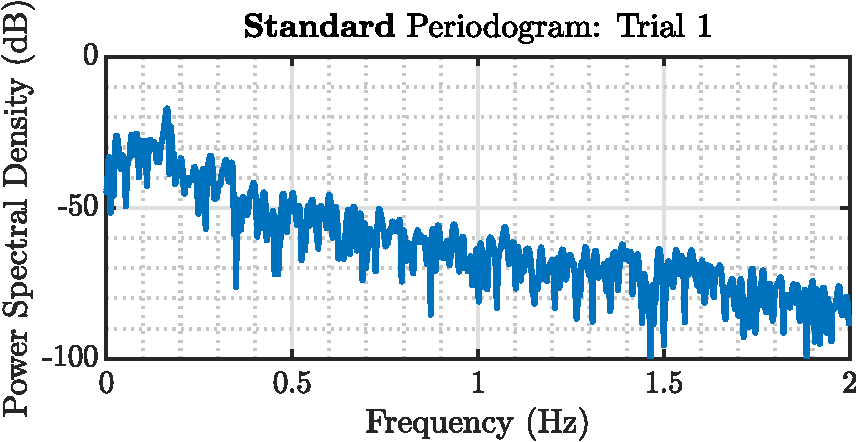
\includegraphics[height=1.5in]{report/parametric-and-line-spectra/real-world-signals_respiratory-sinus-arrhythmia-from-RR-Intervals/assets/a/standard-trial1}
    \end{subfigure}
    ~
    \begin{subfigure}{0.49\textwidth}
        \centering
        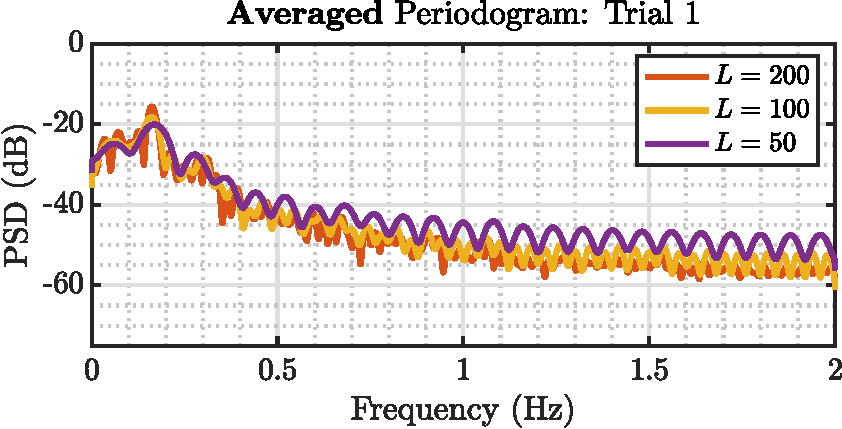
\includegraphics[height=1.5in]{report/parametric-and-line-spectra/real-world-signals_respiratory-sinus-arrhythmia-from-RR-Intervals/assets/a/averaged-trial1}
    \end{subfigure}
    ~
    ~
    \begin{subfigure}{0.49\textwidth}
        \centering
        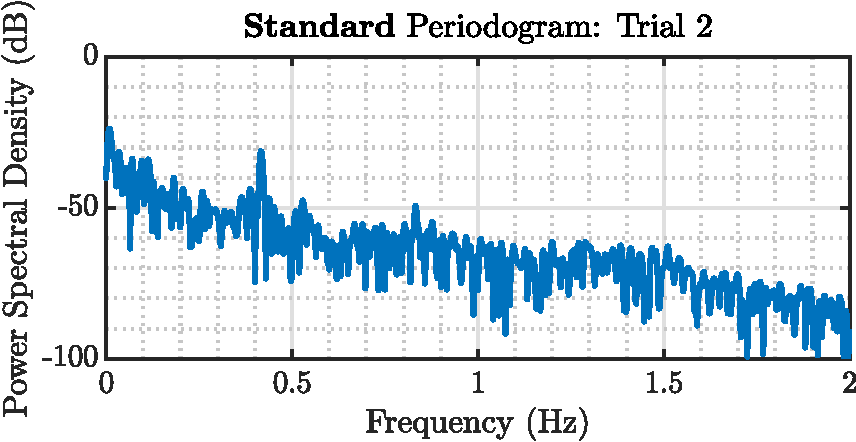
\includegraphics[height=1.5in]{report/parametric-and-line-spectra/real-world-signals_respiratory-sinus-arrhythmia-from-RR-Intervals/assets/a/standard-trial2}
    \end{subfigure}
    ~ 
    \begin{subfigure}{0.49\textwidth}
        \centering
        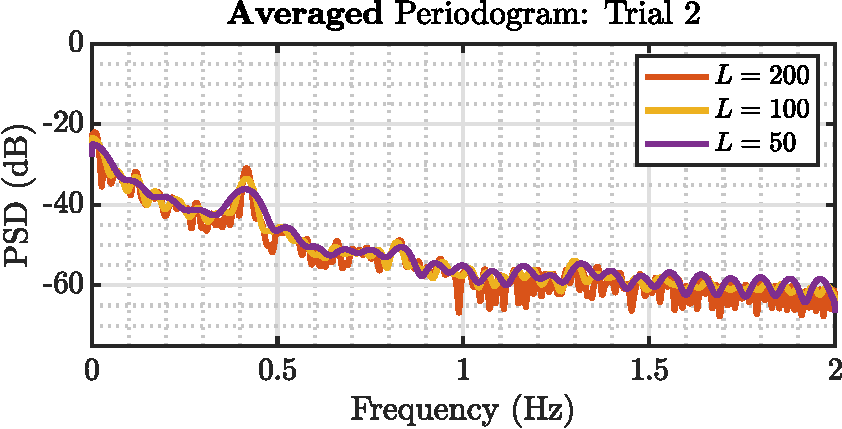
\includegraphics[height=1.5in]{report/parametric-and-line-spectra/real-world-signals_respiratory-sinus-arrhythmia-from-RR-Intervals/assets/a/averaged-trial2}
    \end{subfigure}
    ~
    ~
    \begin{subfigure}{0.49\textwidth}
        \centering
        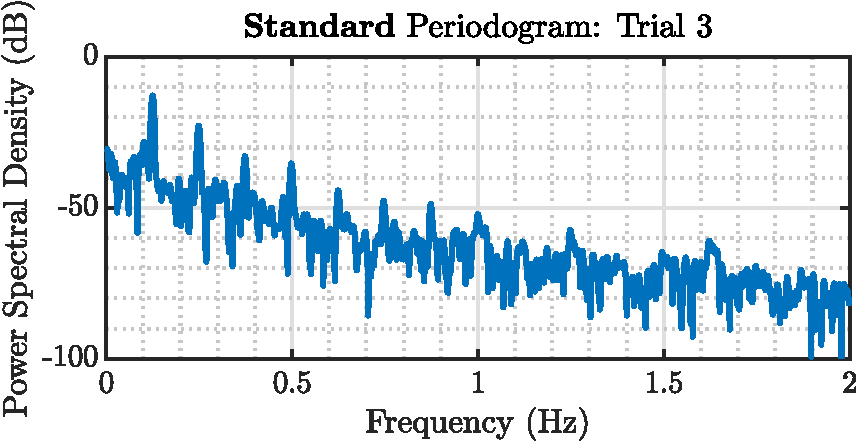
\includegraphics[height=1.5in]{report/parametric-and-line-spectra/real-world-signals_respiratory-sinus-arrhythmia-from-RR-Intervals/assets/a/standard-trial3}
    \end{subfigure}
    ~
    \begin{subfigure}{0.49\textwidth}
        \centering
        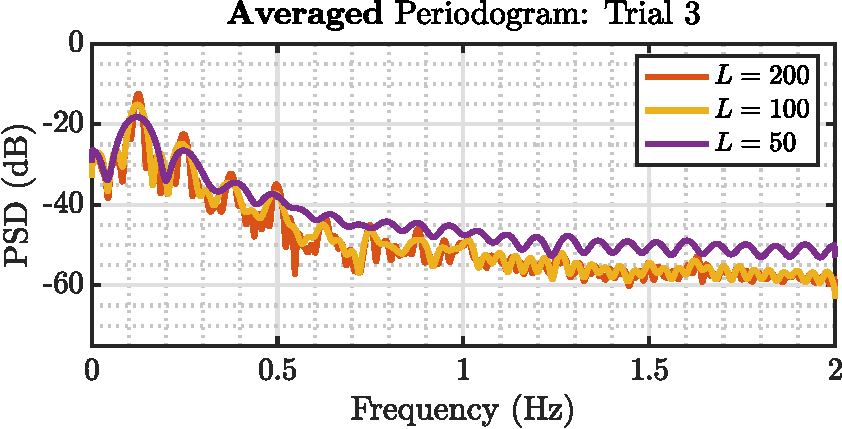
\includegraphics[height=1.5in]{report/parametric-and-line-spectra/real-world-signals_respiratory-sinus-arrhythmia-from-RR-Intervals/assets/a/averaged-trial3}
    \end{subfigure}
    \caption{RRI: standard and averaged periodograms with different window lengths $L$.}
    \label{fig:2_4_a}
\end{figure}

%% b)
\item
%

The three trials were carried out under different breathing conditions, which is reflected by the Breaths per Minute (BPM) rate.
Table \ref{tab:2_4_b} summarises the conditions and the corresponding expected and observed BPM measurements for each trial.

\begin{table}[h]
\centering
\begin{tabular}{|c|c|c||c|}
\hline
& \textbf{Conditions} & \textbf{Expected Range} (BPM) & \textbf{Observation} (BPM) \\
\hline
\hline
\textbf{Trial 1} & normal \& unconstraint breathing & $12 - 35$ & $19.69$ \\
\hline
\textbf{Trial 2} & fast breathing & $35 - 50$ & $49.92$ \\
\hline
\textbf{Trial 3} & slow breathing & $8 - 15$ & $15$ \\
\hline
\end{tabular}
\caption{RRI: conditions and observed BPM.}
\label{tab:2_4_b}
\end{table}

The observed peaks for the three trials are at frequencies $f_{1} = 0.1641\ Hz$, $f_{2} = 0.416\ Hz$ and $f_{3} = 0.125\ Hz$.
For trial 1, both the standard and the averaged periodograms have a peak at $f_{1} = 0.1641\ Hz$, however the averaged periodograms due to their inadequate frequency resolution
fail to capture its harmonics, which are hardly visible also at the standard periodogram. Trial 2 peak at $f_{2} = 0.416\ Hz$ and its second and third harmonics are visible
using any of the provided methods. Lastly, trial 3 peak at $f_{3} = 0.125\ Hz$ and its harmonics are clearly captures by both the standard and the averaged periodograms.

\pagebreak

%% c)
\item
%

The power spectral density of the three trials is estimated by fitting $p$ order AR processes and figures \ref{fig:2_4_c_1}, \ref{fig:2_4_c_2} and \ref{fig:2_4_c_3} are obtained.

\begin{figure}[h]
    \centering
    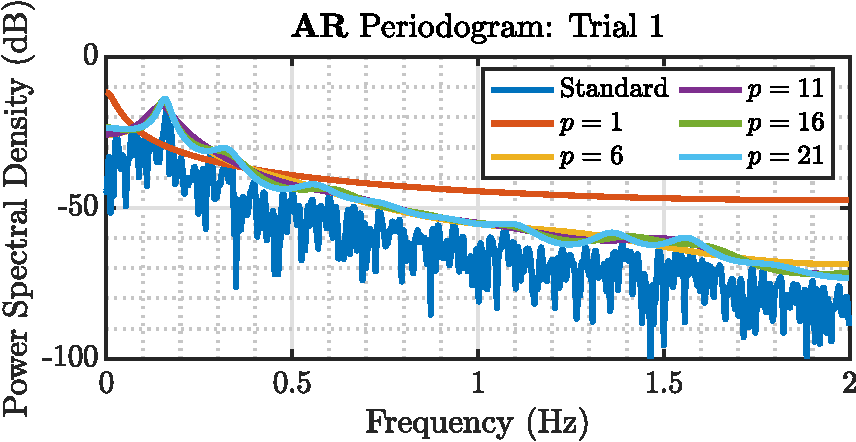
\includegraphics[height=1.5in]{report/parametric-and-line-spectra/real-world-signals_respiratory-sinus-arrhythmia-from-RR-Intervals/assets/c/standard_ar-trial1}
    \caption{RRI Trial 1: AR process spectral estimation.}
    \label{fig:2_4_c_1}
\end{figure}

For trial 1, for $p \geq 11$, the fundamental frequency $f_{1} = 0.1641\ Hz$ and its 3 first harmonics are identified, corraborating with the results of the previous part.

\begin{figure}[h]
    \centering
    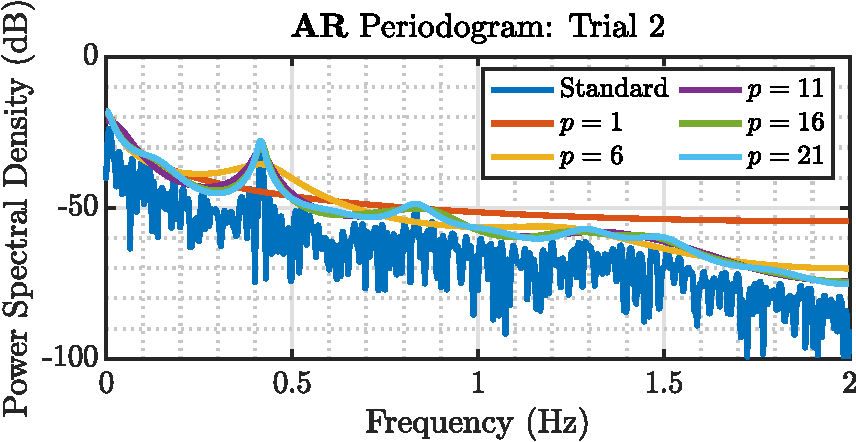
\includegraphics[height=1.5in]{report/parametric-and-line-spectra/real-world-signals_respiratory-sinus-arrhythmia-from-RR-Intervals/assets/c/standard_ar-trial2}
    \caption{RRI Trial 2: AR process spectral estimation.}
    \label{fig:2_4_c_2}
\end{figure}

Figure \ref{fig:2_4_c_2} depicts the AR spectral estimate of trial 2, which again for $p \geq 11$ adequately captures the fundamental frequency and its first three harmonics.

\begin{figure}[h]
    \centering
    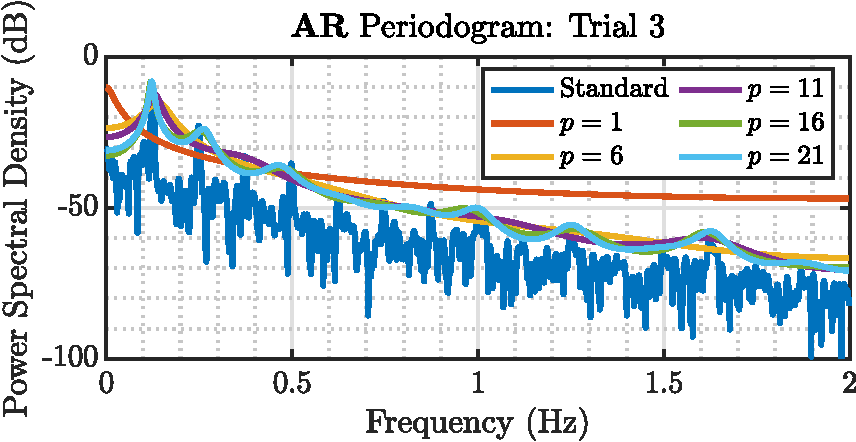
\includegraphics[height=1.5in]{report/parametric-and-line-spectra/real-world-signals_respiratory-sinus-arrhythmia-from-RR-Intervals/assets/c/standard_ar-trial3}
    \caption{RRI Trial 3: AR process spectral estimation.}
    \label{fig:2_4_c_3}
\end{figure}

Last but not least, for $p \geq 16$ trial 3 AR(p) process model discriminated all six first harmonics, verifying the respiration rate reported in the previous part.

Overall, the AR process models can provide reliable estimates when the generative process order $p$ is known, or noise power is negligible compared to the signal power.
When under-modelling is performed ($p < p_{true}$) the estimates cannot identify the frequency peaks, while in presence of noise, over-modelling ($p > p_{true}$) can
lead to overfitting noise and thus providing faulty peaks. Nonetheless, compared to the standard and averaged periodogram methods, the variance, frequency resolution trade-off
is not present in case of AR models.

%
\end{enumerate}